%% bare_jrnl_compsoc.tex
%% V1.3
%% 2007/01/11
%% by Michael Shell
%% See:
%% http://www.michaelshell.org/
%% for current contact information.
%%
%% This is a skeleton file demonstrating the use of IEEEtran.cls
%% (requires IEEEtran.cls version 1.7 or later) with an IEEE Computer
%% Society journal paper.
%%
%% Support sites:
%% http://www.michaelshell.org/tex/ieeetran/
%% http://www.ctan.org/tex-archive/macros/latex/contrib/IEEEtran/
%% and
%% http://www.ieee.org/

%%*************************************************************************
%% Legal Notice:
%% This code is offered as-is without any warranty either expressed or
%% implied; without even the implied warranty of MERCHANTABILITY or
%% FITNESS FOR A PARTICULAR PURPOSE! 
%% User assumes all risk.
%% In no event shall IEEE or any contributor to this code be liable for
%% any damages or losses, including, but not limited to, incidental,
%% consequential, or any other damages, resulting from the use or misuse
%% of any information contained here.
%%
%% All comments are the opinions of their respective authors and are not
%% necessarily endorsed by the IEEE.
%%
%% This work is distributed under the LaTeX Project Public License (LPPL)
%% ( http://www.latex-project.org/ ) version 1.3, and may be freely used,
%% distributed and modified. A copy of the LPPL, version 1.3, is included
%% in the base LaTeX documentation of all distributions of LaTeX released
%% 2003/12/01 or later.
%% Retain all contribution notices and credits.
%% ** Modified files should be clearly indicated as such, including  **
%% ** renaming them and changing author support contact information. **
%%
%% File list of work: IEEEtran.cls, IEEEtran_HOWTO.pdf, bare_adv.tex,
%%                    bare_conf.tex, bare_jrnl.tex, bare_jrnl_compsoc.tex
%%*************************************************************************

% *** Authors should verify (and, if needed, correct) their LaTeX system  ***
% *** with the testflow diagnostic prior to trusting their LaTeX platform ***
% *** with production work. IEEE's font choices can trigger bugs that do  ***
% *** not appear when using other class files.                            ***
% The testflow support page is at:
% http://www.michaelshell.org/tex/testflow/

% Note that the a4paper option is mainly intended so that authors in
% countries using A4 can easily print to A4 and see how their papers will
% look in print - the typesetting of the document will not typically be
% affected with changes in paper size (but the bottom and side margins will).
% Use the testflow package mentioned above to verify correct handling of
% both paper sizes by the user's LaTeX system.
%
% Also note that the "draftcls" or "draftclsnofoot", not "draft", option
% should be used if it is desired that the figures are to be displayed in
% draft mode.
%
% The Computer Society usually requires 12pt for submissions.
%
\documentclass[12pt,journal,compsoc]{IEEEtran}
%
% If IEEEtran.cls has not been installed into the LaTeX system files,
% manually specify the path to it like:
% \documentclass[12pt,journal,compsoc]{../sty/IEEEtran}

%private 
\usepackage{color}

%
\def\RED#1{{\color{red}#1}}%
\def\TODO#1{TODO:\RED#1}
\def\TS#1{\AddToContLine{lots}{#1}#1}%
%



% Some very useful LaTeX packages include:
% (uncomment the ones you want to load)


% *** MISC UTILITY PACKAGES ***
%
%\usepackage{ifpdf}
% Heiko Oberdiek's ifpdf.sty is very useful if you need conditional
% compilation based on whether the output is pdf or dvi.
% usage:
% \ifpdf
%   % pdf code
% \else
%   % dvi code
% \fi
% The latest version of ifpdf.sty can be obtained from:
% http://www.ctan.org/tex-archive/macros/latex/contrib/oberdiek/
% Also, note that IEEEtran.cls V1.7 and later provides a builtin
% \ifCLASSINFOpdf conditional that works the same way.
% When switching from latex to pdflatex and vice-versa, the compiler may
% have to be run twice to clear warning/error messages.

% *** CITATION PACKAGES ***
%
\ifCLASSOPTIONcompsoc
  % IEEE Computer Society needs nocompress option
  % requires cite.sty v4.0 or later (November 2003)
  % \usepackage[nocompress]{cite}
\else
  % normal IEEE
  % \usepackage{cite}
\fi
% cite.sty was written by Donald Arseneau
% V1.6 and later of IEEEtran pre-defines the format of the cite.sty package
% \cite{} output to follow that of IEEE. Loading the cite package will
% result in citation numbers being automatically sorted and properly
% "compressed/ranged". e.g., [1], [9], [2], [7], [5], [6] without using
% cite.sty will become [1], [2], [5]--[7], [9] using cite.sty. cite.sty's
% \cite will automatically add leading space, if needed. Use cite.sty's
% noadjust option (cite.sty V3.8 and later) if you want to turn this off.
% cite.sty is already installed on most LaTeX systems. Be sure and use
% version 4.0 (2003-05-27) and later if using hyperref.sty. cite.sty does
% not currently provide for hyperlinked citations.
% The latest version can be obtained at:
% http://www.ctan.org/tex-archive/macros/latex/contrib/cite/
% The documentation is contained in the cite.sty file itself.
%
% Note that some packages require special options to format as the Computer
% Society requires. In particular, Computer Society  papers do not use
% compressed citation ranges as is done in typical IEEE papers
% (e.g., [1]-[4]). Instead, they list every citation separately in order
% (e.g., [1], [2], [3], [4]). To get the latter we need to load the cite
% package with the nocompress option which is supported by cite.sty v4.0
% and later. Note also the use of a CLASSOPTION conditional provided by
% IEEEtran.cls V1.7 and later.

% *** GRAPHICS RELATED PACKAGES ***
%
\ifCLASSINFOpdf
  % \usepackage[pdftex]{graphicx}
  % declare the path(s) where your graphic files are
  % \graphicspath{{../pdf/}{../jpeg/}}
  % and their extensions so you won't have to specify these with
  % every instance of \includegraphics
  % \DeclareGraphicsExtensions{.pdf,.jpeg,.png}
\else
  % or other class option (dvipsone, dvipdf, if not using dvips). graphicx
  % will default to the driver specified in the system graphics.cfg if no
  % driver is specified.
   %\usepackage[dvips]{graphicx}
   \usepackage[dvipdfmx]{graphicx}
  % declare the path(s) where your graphic files are
  % \graphicspath{{../eps/}}
  % and their extensions so you won't have to specify these with
  % every instance of \includegraphics
  % \DeclareGraphicsExtensions{.eps}
\fi
% graphicx was written by David Carlisle and Sebastian Rahtz. It is
% required if you want graphics, photos, etc. graphicx.sty is already
% installed on most LaTeX systems. The latest version and documentation can
% be obtained at: 
% http://www.ctan.org/tex-archive/macros/latex/required/graphics/
% Another good source of documentation is "Using Imported Graphics in
% LaTeX2e" by Keith Reckdahl which can be found as epslatex.ps or
% epslatex.pdf at: http://www.ctan.org/tex-archive/info/
%
% latex, and pdflatex in dvi mode, support graphics in encapsulated
% postscript (.eps) format. pdflatex in pdf mode supports graphics
% in .pdf, .jpeg, .png and .mps (metapost) formats. Users should ensure
% that all non-photo figures use a vector format (.eps, .pdf, .mps) and
% not a bitmapped formats (.jpeg, .png). IEEE frowns on bitmapped formats
% which can result in "jaggedy"/blurry rendering of lines and letters as
% well as large increases in file sizes.
%
% You can find documentation about the pdfTeX application at:
% http://www.tug.org/applications/pdftex

% *** MATH PACKAGES ***
%
%\usepackage[cmex10]{amsmath}
% A popular package from the American Mathematical Society that provides
% many useful and powerful commands for dealing with mathematics. If using
% it, be sure to load this package with the cmex10 option to ensure that
% only type 1 fonts will utilized at all point sizes. Without this option,
% it is possible that some math symbols, particularly those within
% footnotes, will be rendered in bitmap form which will result in a
% document that can not be IEEE Xplore compliant!
%
% Also, note that the amsmath package sets \interdisplaylinepenalty to 10000
% thus preventing page breaks from occurring within multiline equations. Use:
%\interdisplaylinepenalty=2500
% after loading amsmath to restore such page breaks as IEEEtran.cls normally
% does. amsmath.sty is already installed on most LaTeX systems. The latest
% version and documentation can be obtained at:
% http://www.ctan.org/tex-archive/macros/latex/required/amslatex/math/

% *** SPECIALIZED LIST PACKAGES ***
%
\usepackage{algorithm}
\usepackage{algpseudocode}
% algorithmic.sty was written by Peter Williams and Rogerio Brito.
% This package provides an algorithmic environment fo describing algorithms.
% You can use the algorithmic environment in-text or within a figure
% environment to provide for a floating algorithm. Do NOT use the algorithm
% floating environment provided by algorithm.sty (by the same authors) or
% algorithm2e.sty (by Christophe Fiorio) as IEEE does not use dedicated
% algorithm float types and packages that provide these will not provide
% correct IEEE style captions. The latest version and documentation of
% algorithmic.sty can be obtained at:
% http://www.ctan.org/tex-archive/macros/latex/contrib/algorithms/
% There is also a support site at:
% http://algorithms.berlios.de/index.html
% Also of interest may be the (relatively newer and more customizable)
% algorithmicx.sty package by Szasz Janos:
% http://www.ctan.org/tex-archive/macros/latex/contrib/algorithmicx/




% *** ALIGNMENT PACKAGES ***
%
%\usepackage{array}
% Frank Mittelbach's and David Carlisle's array.sty patches and improves
% the standard LaTeX2e array and tabular environments to provide better
% appearance and additional user controls. As the default LaTeX2e table
% generation code is lacking to the point of almost being broken with
% respect to the quality of the end results, all users are strongly
% advised to use an enhanced (at the very least that provided by array.sty)
% set of table tools. array.sty is already installed on most systems. The
% latest version and documentation can be obtained at:
% http://www.ctan.org/tex-archive/macros/latex/required/tools/


%\usepackage{mdwmath}
%\usepackage{mdwtab}
% Also highly recommended is Mark Wooding's extremely powerful MDW tools,
% especially mdwmath.sty and mdwtab.sty which are used to format equations
% and tables, respectively. The MDWtools set is already installed on most
% LaTeX systems. The lastest version and documentation is available at:
% http://www.ctan.org/tex-archive/macros/latex/contrib/mdwtools/


% IEEEtran contains the IEEEeqnarray family of commands that can be used to
% generate multiline equations as well as matrices, tables, etc., of high
% quality.

\usepackage{multirow}


%\usepackage{eqparbox}
% Also of notable interest is Scott Pakin's eqparbox package for creating
% (automatically sized) equal width boxes - aka "natural width parboxes".
% Available at:
% http://www.ctan.org/tex-archive/macros/latex/contrib/eqparbox/





% *** SUBFIGURE PACKAGES ***
\ifCLASSOPTIONcompsoc
\usepackage[tight,normalsize,sf,SF]{subfigure}
\else
\usepackage[tight,footnotesize]{subfigure}
\fi
% subfigure.sty was written by Steven Douglas Cochran. This package makes it
% easy to put subfigures in your figures. e.g., "Figure 1a and 1b". For IEEE
% work, it is a good idea to load it with the tight package option to reduce
% the amount of white space around the subfigures. Computer Society papers
% use a larger font and \sffamily font for their captions, hence the
% additional options needed under compsoc mode. subfigure.sty is already
% installed on most LaTeX systems. The latest version and documentation can
% be obtained at:
% http://www.ctan.org/tex-archive/obsolete/macros/latex/contrib/subfigure/
% subfigure.sty has been superceeded by subfig.sty.


%\ifCLASSOPTIONcompsoc
%  \usepackage[caption=false]{caption}
%  \usepackage[font=normalsize,labelfont=sf,textfont=sf]{subfig}
%\else
%  \usepackage[caption=false]{caption}
%  \usepackage[font=footnotesize]{subfig}
%\fi
% subfig.sty, also written by Steven Douglas Cochran, is the modern
% replacement for subfigure.sty. However, subfig.sty requires and
% automatically loads Axel Sommerfeldt's caption.sty which will override
% IEEEtran.cls handling of captions and this will result in nonIEEE style
% figure/table captions. To prevent this problem, be sure and preload
% caption.sty with its "caption=false" package option. This is will preserve
% IEEEtran.cls handing of captions. Version 1.3 (2005/06/28) and later 
% (recommended due to many improvements over 1.2) of subfig.sty supports
% the caption=false option directly:
%\ifCLASSOPTIONcompsoc
%  \usepackage[caption=false,font=normalsize,labelfont=sf,textfont=sf]{subfig}
%\else
%  \usepackage[caption=false,font=footnotesize]{subfig}
%\fi
%
% The latest version and documentation can be obtained at:
% http://www.ctan.org/tex-archive/macros/latex/contrib/subfig/
% The latest version and documentation of caption.sty can be obtained at:
% http://www.ctan.org/tex-archive/macros/latex/contrib/caption/




% *** FLOAT PACKAGES ***
%
%\usepackage{fixltx2e}
% fixltx2e, the successor to the earlier fix2col.sty, was written by
% Frank Mittelbach and David Carlisle. This package corrects a few problems
% in the LaTeX2e kernel, the most notable of which is that in current
% LaTeX2e releases, the ordering of single and double column floats is not
% guaranteed to be preserved. Thus, an unpatched LaTeX2e can allow a
% single column figure to be placed prior to an earlier double column
% figure. The latest version and documentation can be found at:
% http://www.ctan.org/tex-archive/macros/latex/base/



%\usepackage{stfloats}
% stfloats.sty was written by Sigitas Tolusis. This package gives LaTeX2e
% the ability to do double column floats at the bottom of the page as well
% as the top. (e.g., "\begin{figure*}[!b]" is not normally possible in
% LaTeX2e). It also provides a command:
%\fnbelowfloat
% to enable the placement of footnotes below bottom floats (the standard
% LaTeX2e kernel puts them above bottom floats). This is an invasive package
% which rewrites many portions of the LaTeX2e float routines. It may not work
% with other packages that modify the LaTeX2e float routines. The latest
% version and documentation can be obtained at:
% http://www.ctan.org/tex-archive/macros/latex/contrib/sttools/
% Documentation is contained in the stfloats.sty comments as well as in the
% presfull.pdf file. Do not use the stfloats baselinefloat ability as IEEE
% does not allow \baselineskip to stretch. Authors submitting work to the
% IEEE should note that IEEE rarely uses double column equations and
% that authors should try to avoid such use. Do not be tempted to use the
% cuted.sty or midfloat.sty packages (also by Sigitas Tolusis) as IEEE does
% not format its papers in such ways.




%\ifCLASSOPTIONcaptionsoff
%  \usepackage[nomarkers]{endfloat}
% \let\MYoriglatexcaption\caption
% \renewcommand{\caption}[2][\relax]{\MYoriglatexcaption[#2]{#2}}
%\fi
% endfloat.sty was written by James Darrell McCauley and Jeff Goldberg.
% This package may be useful when used in conjunction with IEEEtran.cls'
% captionsoff option. Some IEEE journals/societies require that submissions
% have lists of figures/tables at the end of the paper and that
% figures/tables without any captions are placed on a page by themselves at
% the end of the document. If needed, the draftcls IEEEtran class option or
% \CLASSINPUTbaselinestretch interface can be used to increase the line
% spacing as well. Be sure and use the nomarkers option of endfloat to
% prevent endfloat from "marking" where the figures would have been placed
% in the text. The two hack lines of code above are a slight modification of
% that suggested by in the endfloat docs (section 8.3.1) to ensure that
% the full captions always appear in the list of figures/tables - even if
% the user used the short optional argument of \caption[]{}.
% IEEE papers do not typically make use of \caption[]'s optional argument,
% so this should not be an issue. A similar trick can be used to disable
% captions of packages such as subfig.sty that lack options to turn off
% the subcaptions:
% For subfig.sty:
% \let\MYorigsubfloat\subfloat
% \renewcommand{\subfloat}[2][\relax]{\MYorigsubfloat[]{#2}}
% For subfigure.sty:
% \let\MYorigsubfigure\subfigure
% \renewcommand{\subfigure}[2][\relax]{\MYorigsubfigure[]{#2}}
% However, the above trick will not work if both optional arguments of
% the \subfloat/subfig command are used. Furthermore, there needs to be a
% description of each subfigure *somewhere* and endfloat does not add
% subfigure captions to its list of figures. Thus, the best approach is to
% avoid the use of subfigure captions (many IEEE journals avoid them anyway)
% and instead reference/explain all the subfigures within the main caption.
% The latest version of endfloat.sty and its documentation can obtained at:
% http://www.ctan.org/tex-archive/macros/latex/contrib/endfloat/
%
% The IEEEtran \ifCLASSOPTIONcaptionsoff conditional can also be used
% later in the document, say, to conditionally put the References on a 
% page by themselves.




% *** PDF, URL AND HYPERLINK PACKAGES ***
%
%\usepackage{url}
% url.sty was written by Donald Arseneau. It provides better support for
% handling and breaking URLs. url.sty is already installed on most LaTeX
% systems. The latest version can be obtained at:
% http://www.ctan.org/tex-archive/macros/latex/contrib/misc/
% Read the url.sty source comments for usage information. Basically,
% \url{my_url_here}.

\hyphenation{op-tical net-works semi-conduc-tor}


\begin{document}
\title{Coordinating CPU and GPU Resources with Loadable Real-Time Schedulers}
\author{
Yusuke~Fujii,~\IEEEmembership{Member,~IEEE,}
Takuya~Azumi,~\IEEEmembership{Member,~IEEE,}
Nobuhiko~Nishio,~\IEEEmembership{Member,~IEEE,}
Tsuyoshi~Hamada, ~\IEEEmembership{Member,~IEEE,}
Shinpei~Kato,~\IEEEmembership{Member,~IEEE,}
\IEEEcompsocitemizethanks{
\IEEEcompsocthanksitem Y. Fujii is with the Graduate School of Information Science and Engineering, Ritsumeikan University.
\IEEEcompsocthanksitem T. Azumi is with the Graduate School of Information Science and Engineering, Osaka University.
\IEEEcompsocthanksitem N. Nishio is with the College of Information Science and Engineering, Ritsumeikan University.
\IEEEcompsocthanksitem T. Hamada is with the Advanced Computing Center, University of Nagasaki.
\IEEEcompsocthanksitem S. Kato is with the School of Information Science, Nagoya University.
}}

% The paper headers
\markboth{Journal of \LaTeX\ Class Files,~Vol.~6, No.~1, January~2007}%
{Shell \MakeLowercase{\textit{et al.}}: Bare Demo of IEEEtran.cls for Computer Society Journals}
% The only time the second header will appear is for the odd numbered pages
% after the title page when using the twoside option.
% 
% *** Note that you probably will NOT want to include the author's ***
% *** name in the headers of peer review papers.                   ***
% You can use \ifCLASSOPTIONpeerreview for conditional compilation here if
% you desire.



% The publisher's ID mark at the bottom of the page is less important with
% Computer Society journal papers as those publications place the marks
% outside of the main text columns and, therefore, unlike regular IEEE
% journals, the available text space is not reduced by their presence.
% If you want to put a publisher's ID mark on the page you can do it like
% this:
%\IEEEpubid{0000--0000/00\$00.00~\copyright~2007 IEEE}
% or like this to get the Computer Society new two part style.
%\IEEEpubid{\makebox[\columnwidth]{\hfill 0000--0000/00/\$00.00~\copyright~2007 IEEE}%
%\hspace{\columnsep}\makebox[\columnwidth]{Published by the IEEE Computer Society\hfill}}
% Remember, if you use this you must call \IEEEpubidadjcol in the second
% column for its text to clear the IEEEpubid mark (Computer Society jorunal
% papers don't need this extra clearance.)



% use for special paper notices
%\IEEEspecialpapernotice{(Invited Paper)}



% for Computer Society papers, we must declare the abstract and index terms
% PRIOR to the title within the \IEEEcompsoctitleabstractindextext IEEEtran
% command as these need to go into the title area created by \maketitle.
\IEEEcompsoctitleabstractindextext{%
\begin{abstract}
%\boldmath
Graphics processing units (GPUs) easily provide the benefits of high-performance computing.
However, GPUs runtime environment is target to best-effort oriented application, and do not consider real-time.
Previous work have contributed for real-time GPU, and depends kernel.
Dependence on the kernel and the device driver gives the burden developers and users.
We present Linux-RTXG which is cordinating CPU and GPU resources for real-time extending framework without kernel modification by loadable kernel modules approach. 
Linux-RTXG has a CPU real-time scheduler, a GPU real-time scheduler, and a GPU reservation mechanism.
To achieve framework without kernel modification, 
we presents interrupt intercept mechanisms and independent interrupt mechanisms and to solved currently Linux kernel real-time scheduling problem.
Experimental results indicate that overhead of GPU scheduling using Linux-RTXG framework,
and kernel free's approach performances of QoS management had kept equivalent performance as compared with the existing kernel-dependent approach.


\end{abstract}
% IEEEtran.cls defaults to using nonbold math in the Abstract.
% This preserves the distinction between vectors and scalars. However,
% if the journal you are submitting to favors bold math in the abstract,
% then you can use LaTeX's standard command \boldmath at the very start
% of the abstract to achieve this. Many IEEE journals frown on math
% in the abstract anyway. In particular, the Computer Society does
% not want either math or citations to appear in the abstract.

% Note that keywords are not normally used for peerreview papers.
\begin{IEEEkeywords}
Computer Society, IEEEtran, journal, \LaTeX, paper, template.
\end{IEEEkeywords}}


% make the title area
\maketitle


% To allow for easy dual compilation without having to reenter the
% abstract/keywords data, the \IEEEcompsoctitleabstractindextext text will
% not be used in maketitle, but will appear (i.e., to be "transported")
% here as \IEEEdisplaynotcompsoctitleabstractindextext when compsoc mode
% is not selected <OR> if conference mode is selected - because compsoc
% conference papers position the abstract like regular (non-compsoc)
% papers do!
\IEEEdisplaynotcompsoctitleabstractindextext
% \IEEEdisplaynotcompsoctitleabstractindextext has no effect when using
% compsoc under a non-conference mode.


% For peer review papers, you can put extra information on the cover
% page as needed:
% \ifCLASSOPTIONpeerreview
% \begin{center} \bfseries EDICS Category: 3-BBND \end{center}
% \fi
%
% For peerreview papers, this IEEEtran command inserts a page break and
% creates the second title. It will be ignored for other modes.
\IEEEpeerreviewmaketitle

../linux-rtx/introduction.tex
\section{System Model}\label{sec:system_model}
In this section, we explain GPU task model on this paper while we discuss the GPU scheduling question and prior work.
Next, we make available limitation for clearing the implementation of no patched GPU scheduling.
This paper focus on a system composed of multiple GPU and multi-core CPU.

\subsection{GPU Task Model}
In case of  General Purpose GPU computing (GPGPU), CUDA and OpenCL are used to implement GPU applications.
This paper focuses on CUDA, but it is possible to adapt the same approach to OpenCL.

We define a GPU task which is to execute the GPU using process,
and a GPU kernel that is unit of processing to executed on the GPU side.
GPU application enclosed multiple GPU tasks.

GPUs are used a set of the API supported by the runtime environment such as CUDA,
typically GPU application taking the following steps:
(i) \textit{cuCtxCreate} creates a GPU context,
(ii) \textit{cuMemAlloc} allocate spaces to device memory, 
(iii) \textit{cuModuleLoad} and \textit{cuMemcpyHtoD} copie the data and the GPU kernel to the allocated device memory spaces from host memory spaces,
(iv) \textit{cuLaunchGrid} launch the GPU kernel, 
(v) \textit{cuCtxSynchronize} is to synchronize waiting kernel is completion, 
(vi) \textit{cuMemcpyDtoH} transfer resultant datas to host memory from device memory, and
(vii) \textit{cuMemFree}, \textit{cuModuleUnload}, and \textit{cuCtxDestroy} release allocated memory spaces and the GPU context.


%我々は本稿においては、GPU実行が少しでも含まれるプロセスであり、ある事柄を成し遂げる一つの単位をアプリケーションとする。 (e.g. pedestrian detection application).
%またこの一連の流れによってGPUを実行する1プロセスをGPUタスクとし、
%GPU側で実行されるカーネルをGPUカーネルと定義する。

\subsection{GPU Scheduling}
A real-time OS (RTOS) is a lot of research~\cite{spring, redline,itron,rk} has been conducted for a long time.
In among them have also been many studies~\cite{litmus,prk,rtai,yodaiken1999rtlinux,kato2009loadable} real-time OS, which is based on the Linux.
%リアルタイムOSは古来より多くの研究~\cite{spring,redline,itron,rk}が行われてきている。
%LinuxをベースとしたリアルタイムOSとしても数多く研究~\cite{prk,rtai,yodaiken1999rtlinux,litmus,kato:loadable}されている。
%GPUを利用可能な環境はWindows, Mac OS, Linuxと限られており、リアルタイムという性質を追求するためにはLinuxの利用が最適であるため、今回我々はlinuxを利用する。
OS available the GPU is limited to Windows, Mac OS and Linux,
we selected Linux in order to achieve real-time on GPU environments.

In order to meet real-time constraints on shared resource environment such as multicore environment,
there are two requirements of a scheduler as follows:
%マルチコア環境でリアルタイムを実現するにあたりスケジューラが最低限必要とする要件は以下の2つである.
\begin{itemize}
\item To use resources according to specified order
%.The mechanisms is resources that are available to the specified order
%u指れた順番でリソースが利用可能なこと
\item To limit the use of the shared resource
\end{itemize}
The previous work's basic approach to satisfy the first is priority-based scheduling (e.g. Rate-Monotonic~\cite{sched:rm} and Earliest Deadline First~\cite{sched:edf}) with technique to prevent priority inversion,
and the second is resource reservation based scheduling (e.g. Constant Bandwidth Server~\cite{rr:cbs}, Total Bandwidth Server~\cite{rr:tbs2}).
%これらを満たすための基本的なアプローチとして,一つ目は優先度ベースのスケジューリング (e.g. Rate-monotonic, Earliest deadline first),
%2つ目は,リソースリザベーションベースのスケジューリング (e.g. CBS, TBS, credit)が用いられる.
GPUs are need to handle a data transfer bandwidth and a processing core as a shared resource,
therefore, we satisfy the two requirements similar to above multicore environment.
%GPUはデータ転送帯域,プロセッシングコアの2つを共有リソースとして扱う必要性があり,上記マルチコア環境と同様に2つの要件を満たす必要がある.
%Therefore, in the system of including GPU is 
%そのためGPUが含まれるシステムにおいても,リアルタイムを実現するためには上記二点を達成できればよい.
Our previous working only to scheduling GPU accesses.
However, GPU kernel is driven by API is issued a GPU task,
to truly support  the real-time scheduling, it is need to schedule a GPU task;
therefore, for realized real-time GPU, framework need to have CPU's priority-based scheduler, GPU's priority-based scheduler and restrict GPU resource by resource reservation mechanisms.
%我々がこれまで取り組んできたGPUリソースマネージメントに関する研究では,
%GPUへのアクセスのみをスケジューリングしてきた.
%しかしながらGPUカーネルはGPUタスクから発行されるAPIを起点に動作していることから,
%真にリアルタイムスケジューリングを適応するためには,GPUタスク自体のスケジューリングを行う必要がある.
%したがって,GPUをリアルタイムにスケジューリングするために必要なメカニズムは,
%CPUの優先度ベーススケジューラ,GPUの優先度ベーススケジューラ,リソースリザベーションによるGPUリソース制限である.
Recently, GPUSync is to work the above interdependence of CPU scheduler and GPU scheduler.
%最近ではGPUSyncが上記のCPUスケジューラとGPUスケジューラの相互依存について取り組んでいる.

%しかし,GPUSyncは$LITMUS^RT$に依存しており,パッチによるインストレーションを必要とする.
%Section~\ref{sec:intro}で述べたとおり,カーネルにパッチを当てる作業は大きな負担になる.
GPUs have some problems on using real-time environment, except  scheduling mechanisms.
GPUs runtime environments are black-box mechanisms results from GPU environments are provided only GPU vendors, and these environments are closed-source.
TimeGraph, Gdev, and RGEM are solve this problem by ensure transparency using reverse engineering and an open-source driver.
GPUSync is solved closed-source compatible by GPU resource management that approaches are the interrupt handling and the runtime access to single.
%GPUのリアルタイム活用にはスケジューリングメカニズム以外の面でも多くの問題がある.
%まずGPUの実行環境がベンダーから提供されるのみであり,クローズドソースになっていることからブラックボックスであることである.
%本問題についてはTIMEGRAPH,GDEV,RGEMではリバースエンジニアリングとオープンソースドライバによって透明性を確保している.
%GPUSyncではランタイムドライバへのアクセスを単一に制限することで,ランタイムドライバが行う資源管理をスルーしている.

The other problem occurs by non-preemptive GPU executions and non-preemptive data transfers.
Several researches~\cite{basaran:preemptive,sparc} realize improvement  the response time by preventing divides the kernel overrun.
%GPUの実行やデータ転送がノンプリエンプティブであることも大きな問題だ.いくつかの研究~\cite{}ではカーネルを分割することで,
%ノンプリエンプティブに起因するオーバランを防ぎ,レスポンスタイムの向上を実現している.
%As these core problems are on the process of being resolved,
However, real-time GPU is experimental-phase while have problem for practical realized.
%このようにいくつかのコアな問題は解決に近づいているが,未だリアルタイムGPUは実験フェーズであり,実用化に向けるには問題が存在している.
The most difficult problem is self-suspending due to GPU is treated as an I/O device.
GPU tasks suspend until it receives the results from issuing the processing to GPU, referred to as self-suspension.
%GPUを完全にリアルタイムに扱うことができないもっとも困難な問題は,GPUがI/Oデバイスとして扱われることに起因する.
%GPUに処理を発行し,結果を受け取るまでの間,発行したタスクは自らサスペンドする.
The self-suspension has been proven as a cause the NP-HARD problem in previous work~\cite{self-sus:1,self-sus:2},
several researches~\cite{chattopadhyay2014limited,kim2013segment} are working on the scheduling analysis for self-suspension task, but it has not been solved yet to complete.

Hence, scheduling framework for the expansion and installation to aim in this study and easy is useful,
it is argued that there is a demand.
%このself-suspensionはこれまでの研究~\cite{self-sus:1,self-sus:2}でNP-HARDな問題を発生させるとして証明されており,
%これまでも多くの研究が執り行われている~\cite{chattopadhyay2014limited,kim2013segment}が,実用レベルでは未だ解決されていない問題である.
%そのため本研究で目指すような拡張,インストールを容易とするスケジューリングフレームワーク実験レベル,実用レベルの両者において有用であり,需要が発生すると推測する.

\textbf{GPU Synchronization:}
%GPUを利用するシステムのようなヘテロジニアス且つメモリを共有しない場合に大きな課題となるのが同期である
The synchronization matters for GPU system such as heterogeneous platoform.
GPU have two different synchronization techniques.
The first techniques is memory map based synchronization which is called FENCE,
it sends GPU commands after the command to take action,
then GPU microcontrollers will write the any value to memory-mapped space after action is completed.
A GPU task monitors it mapped space value using such as polling,
therefore task has an exclusive CPU resource,
but response time will be the fastest.
The other one techniques is interrupts based synchronization which is called NOTIFY,
it sends GPU commands similar to FENCE,
then GPU microcontrollers will rise the interrupt and write any value to GPU I/O registers.
A GPU task is suspending until interrupt,
therefore task is able to share the CPU resources with other tasks,
but response time will be the slow. Detailed architecture is omitted in this paper,
it has been described in the previous documents~\cite{kato:timegraph, kato:gdev, fujii:apsys2013}.

Gdev use both techniques that are NOTIFY and FENCE for wakeup the waiting task,
NOTIFY is used by scheduler, FENCE is used by kernel synchronization. 
Gdev’s synchronization implementation is the additional commands sends to GPU and the modification of device driver’s interrupt handler.
GPUSync use NOTIFY techniques by using tasklet intercept~\cite{elliott2012robust} on the proprietary software.
Tasklet is linux’s soft-irq implementation.
GPUSync identify the interrupt that is issued which kernel by callback pointer with a tasklet.

\textbf{kernel free scheduler:}
To achieve ”kernel free”,
we must not to modify the kernel code and the device driver code.
GPU scheduler is required to receive notify the completion of GPU kernel, for selection of next executing GPU kernel.
It is realized by two methods that are API-driven method and Interrupt-driven method.
The API-driven method is explicitly wakeup the scheduler after the synchronized by API such as $cuCtxSynchronize()$ is provided runtime in the RGEM.
The Interrupt-driven method is wakeup by trigger of the interrupt which is issued by using NOTIFY in the Gdev and TimeGraph.
General utilized $cuCtxSynchronize()$ synchronize completion of all GPU kernels, therefore, API driven is able to use when a GPU context have issued only single kernel.
Thus if a GPU context issue multiple kernels, we must use the Interrupt-driven method for not to guarantee overrun due to reduction of the response time.

%GPU スケジューラは次に実行するカーネルの 選択のために,
%現在実行中のカーネルの実行が終了したという通知を受け取る必要がある.
%この受 取には,API-driven と Interrupt-driven な方式が ある.RGEM ではこの API-driven を用いており, cuCtxSynchronize() などのランタイムによって 提供される API によってカーネルが同期された後 に,明示的にスケジューラを起動する API を発行 する.Gdev や TimeGraph では Interrupt-driven を利用しており,NOTIFY を利用する際に発行さ れる割込みをトリガーとしてスケジューラを起動 する.
%一般的に用いられる cuCtxSynchroniza() は当 該コンテキストで現在発行されている全てのカー ネルが終了したタイミングで同期する.したがっ て API-driven では一つの GPU コンテキストから は一度に一つのカーネルが発行される場合のみに 対応可能である.
%しかしながら,一つの GPU コンテキストから 連続して複数のカーネルが発行されるケースは, 多々発生すると考えられる. その影響から,カー ネル実行のレスポンスタイムが低下し,オーバラ ンの発生率を高める問題が発生する.
The Interrupt-driven method can be synchronized for each kernel, it is required to modification the kernel or the device driver's ISR.
Gdev has been achieved independent synchronization mechanisms on the proprietary soft- ware, need to modify the kernel modification.
The challenge is realize independent synchronization mechanisms by kernel free approach.

We define a GPU task which is to execute the GPU using above API flow,
and define a GPU kernel that is unit of processing to executed on the GPU side.
%Interrupt-driven では NOTIFY で用いられる割 込みを取得するため,各カーネル毎に同期が可能 であるため,スケジューリングを考えた場合には 有効であるが,割込みの取得のために,カーネル もしくはデバイスドライバ内の ISR を直接修正す る必要がある.

\SECTION{Design and Implementation}\label{sec:design_imple}
In this section, we present the design and implementation of Linux-RTXG,
which provides a framework of coordinated CPU and GPU resource
management with LKMs.
We describe our approach to GPU scheduling and its integration to CPU
scheduling.
Due to a space constraint, the detail of LKM-based CPU scheduling is
referred to the RESCH project~\cite{kato2009loadable, asberg2012exsched}.

\SUBSECTION{Linux-RTXG}
\begin{figure}[t]
\begin{center}
\ifthesis
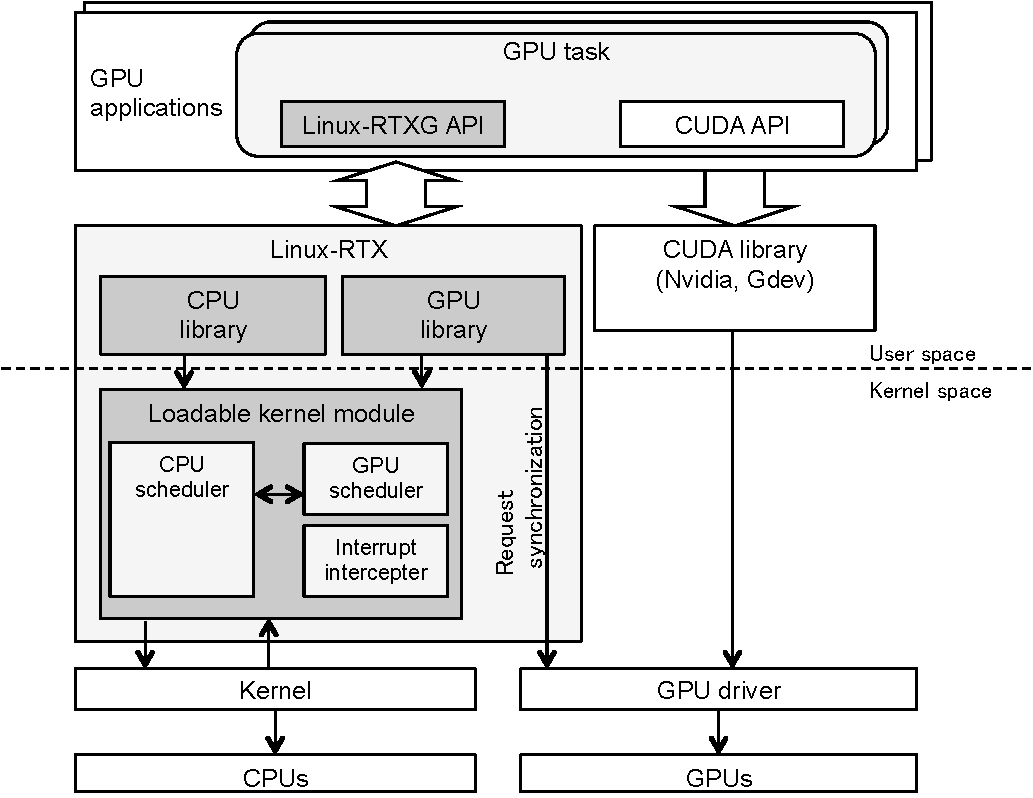
\includegraphics[width=0.8\textwidth]{img/overview.pdf}
\else
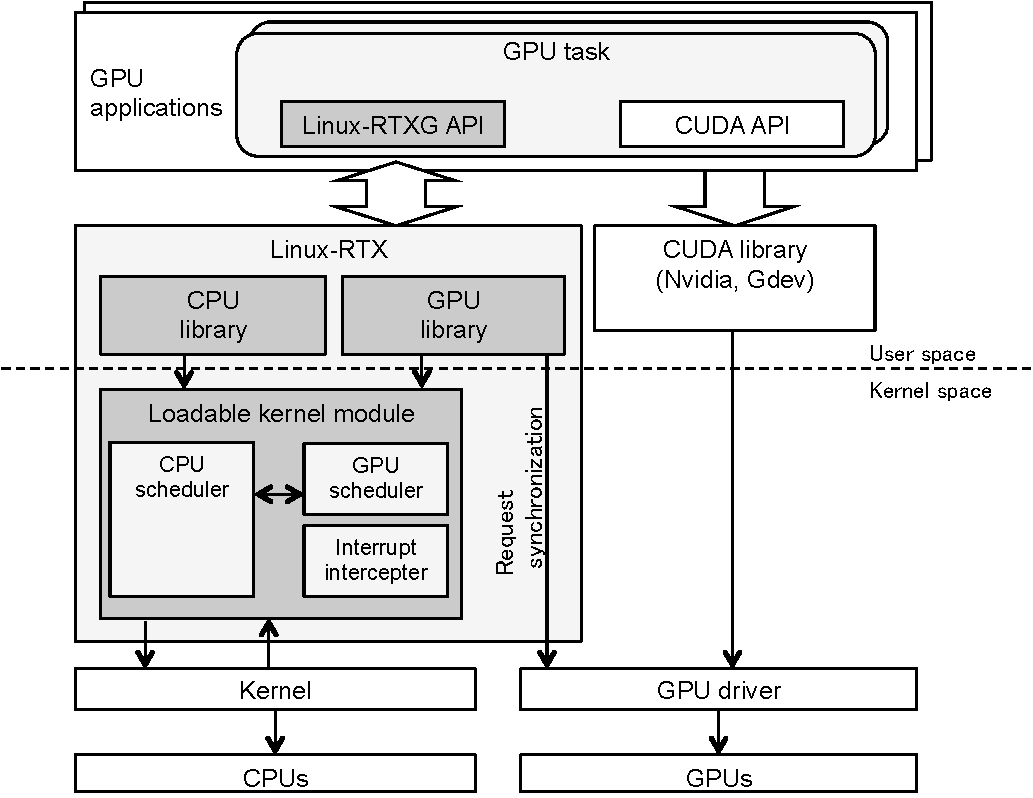
\includegraphics[width=0.35\textwidth]{img/overview.pdf}
\fi
\caption{Architectural overview of Linux-RTXG.}
\label{fig:overview}
\end{center}
\end{figure}

Figure~\ref{fig:overview} shows an architectural overview of
Linux-RTXG.
The system architecture of Linux-RTXG falls into two parts.
First, the Linux-RTXG core contains a CPU scheduler and a GPU scheduler
with a resource reservation mechanism.
The implementation of the Linux-RTXG core is provided in the kernel
space by an LKM.
Thus, it can use exported Linux kernel functions, such as $schedule()$,
$mod\_timer()$, $wake\_up\_process()$, and $set\_cpus\_allowed\_ptr()$.
These functions can be called from the user space interface using the
input/output control (ioctl) system call, which is a standard system
call for device drivers.
Secondly, the Linux-RTXG library contains an independent synchronization
method for coordinated CPU and GPU resource management.
The independent synchronization method can be used on top of a
proprietary driver~\cite{nvidia:cuda_zone} as well as an open-source
driver~\cite{nouveau}.
Note that this method is required to manage interrupts for GPU
scheduling without any code modification to the OS kernel and device
drivers.

\SUBSECTION{GPU Scheduling}
\begin{table*}[!t]
\begin{center}
\caption{A basic set of APIs for Linux-RTXG.}
\label{tab:rtx-api}
\ifthesis
\begin{tabular}{|l|p{25em}|} \hline
\else
\begin{tabular}{|l|p{50em}|} \hline
\fi
rtx\_gpu\_open() & Registers itself to Linux-RTXG and creates scheduling entity. It must be called first. \\ \hline
rtx\_gpu\_device\_advice() & Obtains recommendations for which GPU devices to use. \\ \hline
rtx\_gpu\_launch() & Controls GPU kernel launch timing, (i.e., a scheduling entry point). It must be called before the CUDA launch API. \\ \hline
rtx\_gpu\_sync() & Waits for the completion of GPU kernel execution by sleeping with TASK UNINTERRUPTIBLE status. \\ \hline
rtx\_gpu\_notify() & Sends NOTIFY/FENCE command to GPU. The FENCE/NOTIFY are selected by flag that is set by argument.\\ \hline
rtx\_gpu\_close() & Releases scheduling entity.\\ \hline
\end{tabular}
\end{center}
\end{table*}

Linux-RTXG is based on the interrupt-driven method for GPU
synchronization but is also partly based on the API-driven method.
The scheduler is invoked only when computation requests are submitted.
The basic APIs supported by Linux-RTXG are listed in Table~\ref{tab:rtx-api}.
Note that some APIs have arguments whereas others do not.
Linux-RTXG does not modify the existing CUDA API to cope with
proprietary software, being independent of GPU runtimes. 
However, CUDA application programs must add the Linux-RTXG APIs to use
the functionality of Linux-RTXG.

The sample code including the Linux-RTXG APIs is shown in
Figure~\ref{fig:sample}.
GPU tasks are provided with function calls to Linux-RTXG at strategic
points.

\begin{figure}[!t]
\begin{center}
\begin{tabular}{l}
\hline\hline
{\scriptsize \verb|void gpu_task(){        |}\\
{\scriptsize \verb| /* variable initialization  */        |}\\
{\scriptsize \verb| /* calling RESCH API */        |}\\
{\scriptsize \verb|  dev_id = rtx_gpu_device_advice(dev_id); |}\\
{\scriptsize \verb|  cuDeviceGet(&dev, dev\_id);           |}\\
{\scriptsize \verb|  cuCtxCreate(&ctx, SYNC_FLAG, dev);    |}\\
{\scriptsize \verb|  rtx_gpu_open(&handle, vdev_id);     |}\\
{\scriptsize \verb| /* Module load and set kernel function */ |}\\
{\scriptsize \verb| /* Device memory allocation        */ |}\\
{\scriptsize \verb| /* Memory copy to device from host */ |}\\
{\scriptsize \verb|  rtx_gpu_launch(&handle); |}\\
{\scriptsize \verb|  cuLaunchGrid(function, grid_x, grid_y); |}\\
{\scriptsize \verb|  rtx_gpu_notify(&handle); |}\\
{\scriptsize \verb|  rtx_gpu_sync(&handle);   |}\\
{\scriptsize \verb|  /* Memory copy to host from device */  |}\\
{\scriptsize \verb|  /* Release allocated memory */  |}\\
{\scriptsize \verb|}|}\\
\hline\hline
\end{tabular}
\caption{Sample code with the Linux-RTXG APIs.}
\label{fig:sample}
\end{center}
\end{figure}

\begin{figure}[!t]
\begin{center}
 \ifthesis
 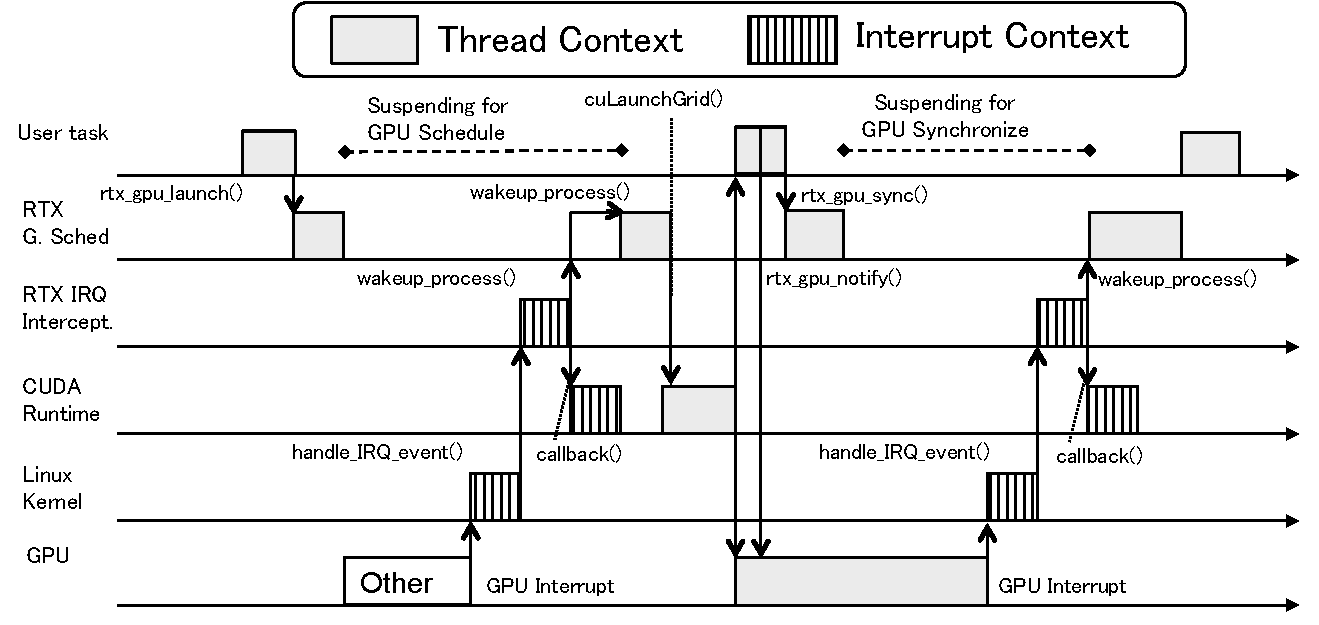
\includegraphics[width=\textwidth]{img/gsched_controlflow.pdf}
 \else
 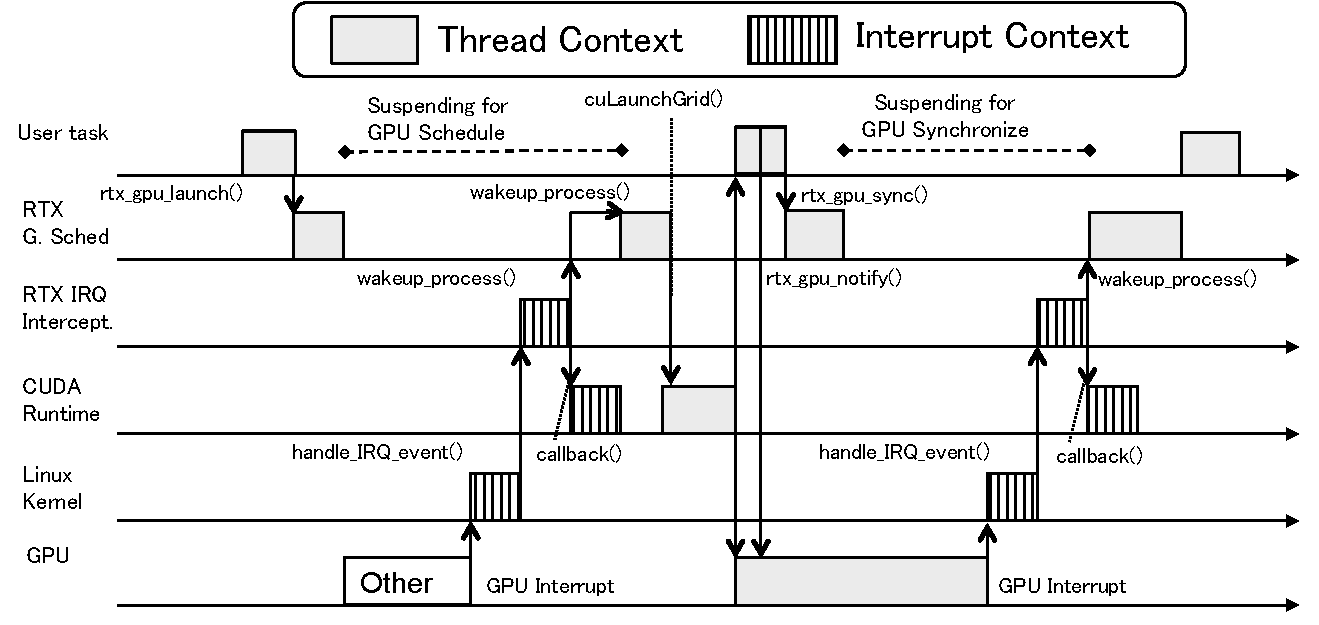
\includegraphics[width=0.5\textwidth]{img/gsched_controlflow.pdf}
 \fi
 \caption{Execution flow of the GPU task.}
 \label{fig:controlflow}
\end{center}
\end{figure}

The execution flow of the GPU task managed by the Linux-RTXG APIs is
described in Figure~\ref{fig:controlflow}.
Note that this example is restricted to a single GPU kernel.
The GPU task can control the timing of GPU kernel invocation by calling
$rtx\_gpu\_launch()$.
After this function call, the task is suspended until it receives an
interrupt so that other GPU kernels can be launched.
When some GPU kernel is completed, an interrupt is raised by the GPU and
the corresponding interrupt handler is executed by the Linux kernel.
The interrupt interceptor awakens some suspending task according to the
priority.
The awakened task proceeds to launch the GPU kernel using the CUDA API,
such as $cuLaunchGrid()$.
After the GPU kernel is launched, the task is going to register NOTIFY
to set up an interrupt, and is again put to the sleep mode until it
receives the interrupt.
Dispatching of the subsequent task is performed by the GPU scheduler,
which is called upon the interrupt from the GPU.
Linux-RTXG manages the order of task execution according to this flow.

We now present a hierarchal scheduling mechanism that uses the concept
of virtual GPUs to combine specified GPU tasks by a group.
The virtual GPUs are realized by a resource reservation mechanism, while
GPU scheduling uses a priority mechanism.
Specifically, each GPU kernel invocation is associated with a scheduling
entity, and Linux-RTXG allocates the scheduling entities to virtual GPUs. 
The virtual GPUs can belong to any physical GPUs.
In Linux-RTXG, computing resources are distributed to virtual GPUs.

Figure~\ref{fig:scheduling} shows the pseudo-code of the Linux-RTXG
scheduler.
This code works under the assumption that $on\_arrival$ is called when
some GPU task requests to launch the GPU kernel.
In $on\_arrival$, the GPU task checks whether the given execution
permission is held by the allocated virtual GPU and is also held by the
allocated scheduling entity.
If the virtual GPU to which the GPU task belongs does not own the
execution permission, the GPU task is enqueued to $wait\_queue$ and is
suspended.
Else, the GPU task can launch the GPU kernel.
After a while, $on\_completion$ is called by the scheduler thread when
the launched GPU kernel is completed, and we can select the next set of
a virtual GPU and a GPU task. 
At the end of $on\_completion$, the selected GPU task is waken up.

\begin{figure}[!t]
\begin{center}
\begin{tabular}{l}
\hline
{\scriptsize \verb| se: The scheduling entity |}\\
{\scriptsize \verb| se->vgpu: The group that belongs to se|}\\
{\scriptsize \verb| se->task: The task that is associated with se |}\\
{\scriptsize \verb| vgpu->parent: The physical GPU identification|}\\
\hline
{\scriptsize \verb|void on_arrival(se) {|}\\
{\scriptsize \verb| check_permit_vgpu(se->vgpu)    |}\\
{\scriptsize \verb| while(!check_permit_se(se)){|}\\
{\scriptsize \verb|   enqueue(se->vgpu,se); |}\\
{\scriptsize \verb|   sleep_task(se->task); |}\\
{\scriptsize \verb|}}|}\\
{\scriptsize \verb|void on_completion(se) {|}\\
{\scriptsize \verb| reset_the_permit(se->vgpu, se)|}\\
{\scriptsize \verb| n_vgpu = pick_up_the_next_vgpu(se->vgpu->parent) |}\\
{\scriptsize \verb| se = pick_up_the_next_se(n_vgpu)|}\\
{\scriptsize \verb| if(se) {|}\\
{\scriptsize \verb|   dequeue(se->vgpu,se);|}\\
{\scriptsize \verb|   wakeup_task(se->task);|}\\
{\scriptsize \verb| }|}\\
{\scriptsize \verb| set_the_permit(se->vgpu, se)|}\\
{\scriptsize \verb|}|}\\
\hline
\end{tabular}
\caption{High-level pseudo-code of the Linux-RTXG scheduler.}
\label{fig:scheduling}
\end{center}
\end{figure}

\SUBSECTION{GPU Synchronization}
Here, we describe the independent synchronization mechanism and the interrupt intercept.
The independent synchronization mechanism invokes NOTIFY and FENCE without using a GPU runtime API.
The interrupt intercept realizes interrupt-driven wakeup of the scheduler without kernel modification.
Linux-RTXG uses the independent synchronization mechanisms as much as possible
because we do not want to use black--box resource management.

\textbf{Independent synchronization mechanism from runtime:}
We present an independent synchronization mechanism for NOTIFY and FENCE.
The mechanism invokes an interrupt for NOTIFY, and writes the fence value with the GPU microcontrollers for FENCE.
NVIDIA's proprietary software uses the ioctl interface to communicate between the kernel-space and the user-space.
These ioctl interfaces provide driver functions, such as device memory allocation, obtaining GPU information and memory mapping.
Gdev builds infrastructure that can execute on NVIDIA's driver using these ioctl interfaces.
The proposed method uses an ioctl interface similar to Gdev's method for sending commands.
Specifically, the proposed method is divided into two parts, Initialize and Notify.
Initialize processess generate a dedicated GPU context.
This processess include creating virtual address space, allocating an indirect buffer object for sending a command, and creating a context object is required to prepare the FIFO engine and includes, allocating a kernel memory object and mapping the FIFO engine register to host memory space using memory-mapped I/O.
The FIFO engine is a GPU microcontroller that receives commands.
The Notify processes send commands to a compute engine or a copy engine by $iowrite$ function to the mapped FIFO engine's register.
The compute engine and the copy engine do function that switching a GPU context for computing or data copy.
This independent synchronization mechanism uses reverse engineering.
Therefore, this method depends on the GPU device architecture and the proprietary software interfaces.

\textbf{Interrupt interception:}
Interrupts are handled by the ISR registered to the kernel by the device driver.
In addition, a scheduler is required to receive the interrupt and to identify the interrupt by reading the GPU status register.
The GPU status register must be read before the original ISR resets the GPU status register.

The Linux kernel has structures that hold interrupt parameters called $irq\_desc$ for each interrupt number.
These structures have structures called $irq\_action$, including the ISR callback pointer.
An $irq\_desc$ is allocated to global kernel memory space, and is freely accessible from kernel space.
Linux loadable kernel modules can obtain an $irq\_desc$ and an ISR callback pointer.
We obtain the GPU device driver's ISR callback pointer, and then we register an interrupt interception ISR to the kernel.
Thus, we obtain an interrupt interception from the interrupt interception ISR and retain the callback pointer.
In addition, I/O registers are mapped to kernel memory space by the device driver from the PCIe base address registers (BAR)~\cite{fujii:icpads2013,kato2013zero}.
Therefore, Linux-RTXG remaps the BAR0 to our allocated space using $ioremap()$ when the ISR initialized.
The interrupt interception identifies an interrupt by reading this mapped-space.

\SUBSECTION{Scheduler Integration}
The native Linux scheduler has various real-time scheduling policies, such as $SCHED\_DEADLINE$, $SCHED\_FIFO$ and $SCHED\_RR$.
$SCHED\_DEADLINE$ is an implementation of a constant bandwidth server and a global earliest deadline first.
$SCHED\_DEADLINE$ is included in the Linux 3.14.0 kernel.
However, synchronization does not work well with the SCHED\_DEADLINE scheduling policy for GPU tasks.
Here there are two problems.
The first is the implementation of $sched\_yield$---.$sched\_yield()$ uses $yield()$ in kernel space---.
The second is the implementation of waking from a sleeping state.

The first problem occurs by releasing the CPU using $sched\_yield()$ while waiting for I/O in polling.
Polling (spin) is the exclusive CPU; therefore, a task may once better to release the CPU can obtain good results.
However, $sched\_yield$ will set the polling task's remaining execution time to 0 by treating it as a parameter of $SCHED\_DEADLINE$.
Thus, the task cannot execute until the runtime is replenished in the next period.
Therefore, the task cannot call $sched\_yield()$ between polling.
$sched yield()$ is frequently used by device drivers and libraries, as well as GPU environment, and such software is affected by this problem.
Depending on the setting, even NVIDIA's CUDA can be affected by this problem.
We address this problem by limiting the GPU synchronization method to NOTIFY in the $SCHED\_DEADLINE$ policies.

The second problem is subjected to a check equation~\ref{eq} when restoring a task from the sleep state.
If equation~\ref{eq} holds, the runtime is replenished and absolute deadline is set to the next cycle deadline.

{\scriptsize
\begin{equation}
\frac{Absolute\_Deadline - Current\_Time}{Remaining\_Runtime} > \frac{Relative\_Deadline}{Period} \label{eq}
\end{equation}
}

We implement this check by subtracting GPU execution time from $Remaining Runtime$ when a task is restored by GPU kernel execution, with the exception of a task that is restored by period.

\section{Evaluation}
We evaluate scheduling overhead and scheduling performance.

Scheduling experiments are limited on the GPU scheduling since CPU scheduling performance is already experiments\cite{kato:resch}.

In this paper, we experiments 

本稿における評価では、本Linux-RTXGを利用した際のオーバヘッドを定量的に計測し、利用に伴ってどれだけのデメリットを含んでいるかを提示する。


\TODO{GPUSyncと比較しなくて良いのか}
\TODO{実アプリで動かすとどうなるのか}

We will discuss in the next chapter for the difference between the functions and features to hold to it with a qualitative evaluation.

%定性的な評価としては関連する研究と保持する機能や特徴の差について次章でdiscussする。

\subsection{Experimental Environment}
Our experiments are conducted with the Linux kernel 3.16.0 on NVIDIA Geforce GTX680 graphics card and 3.40GHz Intel Core i7 2600, which contains 8 cores (including the two hyper-threading cores) and 8GB main memory.
GPU programs are written in CUDA and compiled by NVCC v6.0.1.
GPU drivers are used NVIDIA driver 331.62 and Nouveau driver linux-3.16.0.
CUDA libraries are used NVIDIA CUDA-6.0 and gdev.
%CPUはIntel Core i7 2600 3.40GHz、
%4GB*2のメモリ、GPUはGeForce GTX680を用いる。
%KernelはLinux kernel 3.16.0を用い、ディストリビューションはUbuntu 14.04である。
%CUDAコンパイラはNVCC v6.0.1、CUDAランタイムはcuda-6.0 or Gdev、GPUドライバはNVIDIA (331.62)、Nouveau (linux-3.16.0)を用いる。
%各ランタイム、ドライバは評価項目ごとに使い分ける。

\subsection{Interrupt intercept overhead}
We mesurement overhead due to interrupt interception.
%Interrupt interceptのオーバヘッドの測定を行う。
This experiment use GPU driver which is used the Nouveau in order to compare and identify the type of interrupt.
We compare consumption time from the start ISR until ISR is completion, it consumption time is average time of 1000 times.

%本評価では、GPUドライバはnouveauを用いる。

%割り込み処理は、各割り込みの種類によって、処理時間が異なり、その分布は一様ではないため、単に測定して平均をとっても比較ができない。
%そのため各割り込みの種類の判別のためにNouveauを用いて、割り込みの種類が同一のもので、カーネル内のdo\_IRQ関数内でハンドラが呼ばれてから終了までの時間を測定し
%どの程度のオーバヘッドで割り込みの盗聴及び、盗聴した割り込みがいずれのカーネルに関連したものであるかの識別ができるかどうかを測定する。

\begin{figure}[t]
\begin{center}
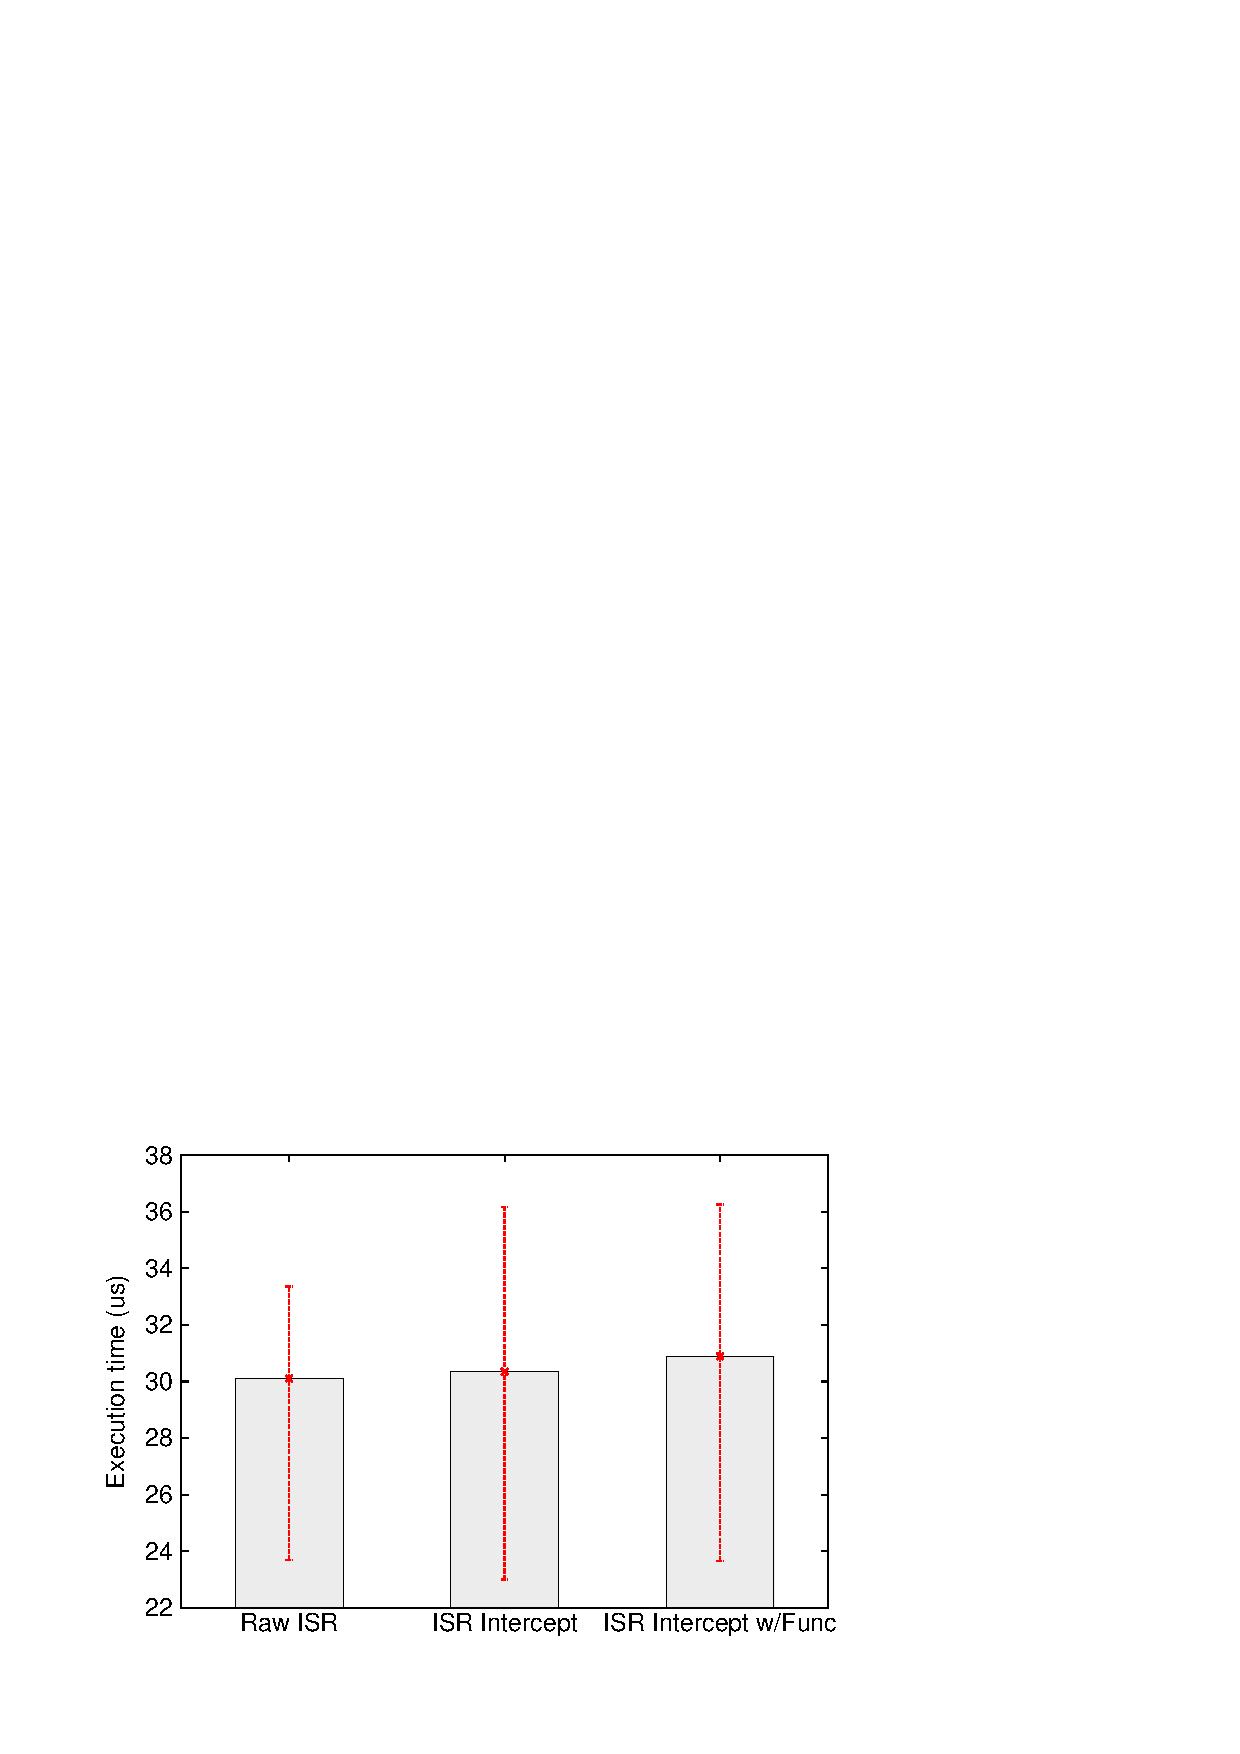
\includegraphics[width=0.4\textwidth]{img/interrupt.pdf}
\caption{Interrupt intercept overhead}
\end{center}
\label{fig:irq_overhead}
\end{figure}

Figure~\ref{irq_overhead} shows results of mesurements in the above setting.
%Figure \ref{irq_overhead}は上記設定で測定した結果である。
Raw ISR is execute ISR in the normal routine, ISR Intercept is only intercept our approach,
ISR intecept w/Func is interception and processing functions that are identify the ISR and wakeup the scheduler thread.
These are showed the average times with error bar is indicate minimum and maximum.

As a result, the overhead exist certainly.
ISR Intercept has overhead that is about 247 nano seconds.
ISR Intercept w/Func also has overhead that is about 790 nano seconds.

Intuitively, it value does not affect system since very small values,
however, interrupt is occured frequently including such as timer interrupt, should be aware as disadvantages.

In addition, we evaluate comparing the response time of the ISR (top-half) and the tasklet (bottom-half) in an environment with noCPU load,
it evaluate does measurement time until the responsible timing from the start of interrupt process which is $do\_IRQ$ function is called).
it mesasurement result is shown in Figure~\ref{fig:bottomvstasklet}.

GPUSync bypass the $tasklet\_schedule()$ if it function is called from the nvidia driver.
The tasklet is generally called after the important procesing in ISR.
It approach has robustness, but response is worse than ISR, it response can be seen from Figure~\ref{fig:bottomvstasklet}.

%Raw ISRは通常のルーチンで実行されるISR、ISR Interceptは割り込みを盗聴するのみ、
%ISR intercept w/Funcは盗聴した上でその割り込みが、いずれのカーネルに関連した割込みか識別しスケジューラを立ち上げる機能を実行した場合である。
%それぞれ1000回の測定で平均値を取り、最小値と最大値についてエラーバーで示している。
%この図から見て取れるように、オーバヘッドは確実に存在する。
%ISR Interceptだと247nsのオーバヘッドであり、
%ISR Intercept w/Funcでも790nsのオーバヘッドである。
%この数値は直感的に考えると小さくシステム自体に影響を及ぼすほどではないと考えられ、
%しかしその割込みが乱発することによる積み重ねによっては影響を与えることは、
%本手法のデメリットとして意識しなければならない。

\subsection{Independent Synchronization mechanism overhead}
We evaluate the overhead according to using independent synchronization mechanism.
The our method is need to call the $rtx\_nvrm\_notify()$ at the timing of requested synchronization (e.g. after the kernel launch issue). 
%本稿では同期生成のためのオーバヘッドを測定する。
%割込みの立ち上げは同期を求めるタイミング(e.g. カーネルラウンチ後)にrtx\_nvrm\_notify()を呼び出す必要がある。
In vanilla environment, these api is not necessary, therefore, time the API consumed is overhead.
%スケジューリングを行わないVanillaな状態ではこれらのAPIは必要ではないものであるため、これらのAPIにかかった時間はすべてオーバヘッドとなる。

We measured overhead by measuring the API consumed time between API call and return.
%そのためこれらのオーバヘッドの計測を行う。計測はAPIの呼び出しから戻るまでを測定する。

\begin{figure}[!t]
\begin{center}
\subfigure[Part of Initialize]{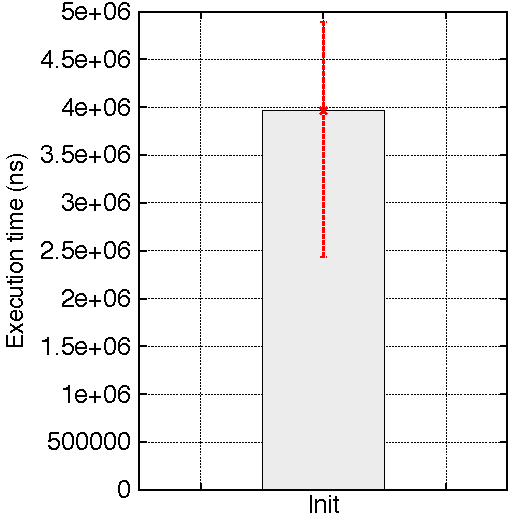
\includegraphics[width=0.23\textwidth]{img/irq_rise_init.pdf}}\subfigure[Part of notify]{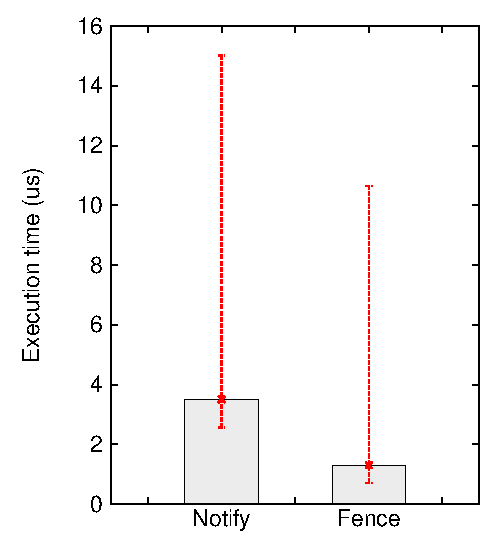
\includegraphics[width=0.23\textwidth]{img/irq_rise_notify.eps}}
\caption{Interrupt raised method overhead}
\label{fig:irq_rise_overhead}
\end{center}
\end{figure}

As a result shown in Figure~\ref{fig:irq_rise_overhead}.
Initialize is need to called the at awaken a linux process for allocating a indirect buffer and register several compute engine to the device driver.
Notify and Fence areGPU command sending to GPU devices which called at timing of the need to synchronization such as after the kernel launch issues.
These methods execution time is variants occurred affected by ioctl system call.
%結果をFigure \ref{fig:irq_rise_overhead}に示す。
%InitializeはIndirect Bufferはプロセスが立ち上がるたびに、
%コマンド送信用のIndirect Bufferの確保や各エンジンの登録のために呼び出される必要がある。
%Notifyはカーネル実行後や非同期メモリコピー実行後のような同期を発生させたいタイミングで呼び出される。
%これらはioctlシステムコールによってユーザ空間とカーネル空間をまたいでる影響か、実行時間のバラ付きが大きく出ている。

Initialize average time is about 4 mill seconds, however, application is not affected too much because above characteristics is only called once.
%Initializeは比較的時間がかかっているが、1プロセスにつき一度しか呼ばれないため、アプリケーション全体への影響は少ないと考えられる。
Notify is not takes much time that is about 3.5µs.
Fence likewise be not takes much time that is about 2µs.
Although may be not have to worry about for most applications,
it is necessary to consider the overhead in a cycle of short application.

\subsection{Scheduling Overhead}\label{sec:eval:sched_overhead}
We will evaluate scheduling overhead by using Linux-RTXG scheduler.
We prepared three applications that are "vanilla", "mutex", and "rtx" for mesurement overheads.
The "rtx" application is scheduled by rtx.
The "mutex" application  is limited to single kernel issue similar to 
rtxでスケジューリングした場合のオーバヘッドを測定するために、"vanilla", "mutex", "rtx"の3種類のアプリケーションを用意した。
全てに共通するのが、1個のアプリケーションに複数のタスクが存在しており、
各タスクには10個のジョブが含まれることである。1個のジョブはGPUへのデータ転送、GPUカーネル実行、GPUからのデータ転送を含んでいる。GPUカーネルは単純な行列の計算を行う。

3種で異なる点として、まずmutexは同時にlaunchが発行されるのが1つに調停されるようにmutexを用いてロックしたバージョンである。
そしてrtxはlinxu-rtxgを用いて実行したケースであり、
vanillaはそれらの追加が無くスケジューリングや調停を一切行わないケースである。

CPUのスケジューリングはlinux-rtxを用いたシンプルなFixed-priorityスケジューリング (LinuxのSCHED\_FIFOと同様のポリシー、ジョブ管理のみを行う)を用いる。
GPU側のスケジューリングは、Gdevで提案されたBANDスケジューラ、Linux-RTXでの同期は全てNOTIFYを用いて行う。

計測結果をFigure~\ref{fig:fp_overhead}に示す。
アプリケーションに含まれるタスク数ごとにプロットしており、各ジョブ内のラウンチ要求から実行完了までにかかった時間の平均値を各処理毎に積み上げ式で示している。


\begin{figure}[t]
\begin{center}
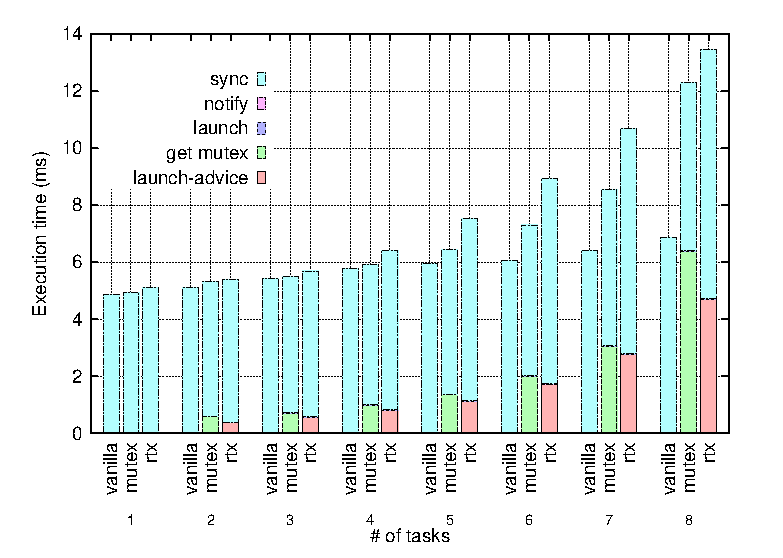
\includegraphics[width=0.5\textwidth]{img/sum_task_fp.eps}
\caption{Scheduling overhead(between GPU kernel launch request and synchronization)}
\end{center}
\label{fig:fp_overhead}
\end{figure}

\TODO{結果について説明と、考察}

launch\_adviceはrtx\_gpu\_launchによってGPU利用のためのリクエストを出してから、許可がでるまでを示しており、
get\_mutexはmutexによってロックを獲得するまでの時間、
launch、notifyはそれぞれコマンドを発行するまでにかかった時間で、
syncは発行されてから同期完了するまでの時間である。
全て、100回のアプリケーション実行($number of tasks ☓$)

\begin{figure}[t]
\begin{center}
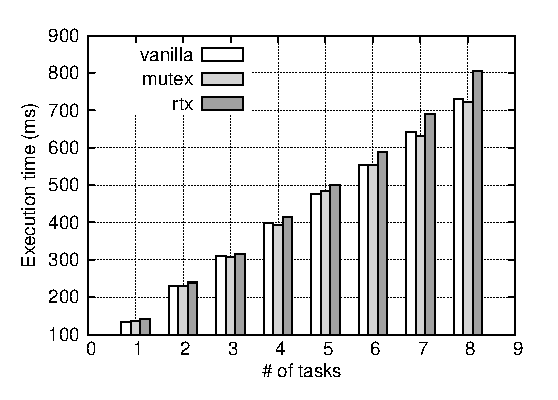
\includegraphics[width=0.5\textwidth]{img/sum_task.eps}
\caption{Scheduling overhead (Time of entire task)}
\end{center}
\label{fig:fp_overhead}
\end{figure}


\subsection{Performance of QoS management}

次にGPUのバジェットエンフォースメントの性能を評価する。
ここでは、今回同一アルゴリズムでQoSマネージメントを行っているGdevとの比較を行い、
パッチを利用しない実装においても、性能をほぼ落とすこと無くできていることを示す。

比較対象は、本Linux-RTXGと同様のスケジューリングアルゴリズムが提供可能なGdevのモジュール版とで比較する。
評価に用いるスケジューリングポリシーはBANDスケジューラを用いる。
実験に利用するアプリケーションとして、\ref{sec:eval:sched_overhead}節で利用したものと同様のものでTaskを4つ生成し、各タスク毎に25\%のGPU利用権限を与える。
これらのタスクの実行中のGPU利用率を計測し、Gdevと同様のアルゴリズムを用いることで、今回提供するLinux−RTXGによるアプローチによってどれだけQoSマネージメントについてのパフォーマンスに影響するかを示す。
Gdevを用いることから、両者ともデバイスドライバはNouveauドライバを用いる.

The first, we experiment the utilization using only priority scheduling, we prepare four diffenre priorities GPU task.
It experiments result show in Figure~\ref{fig:rtx_prio}.

\begin{figure}[t]
\begin{center}
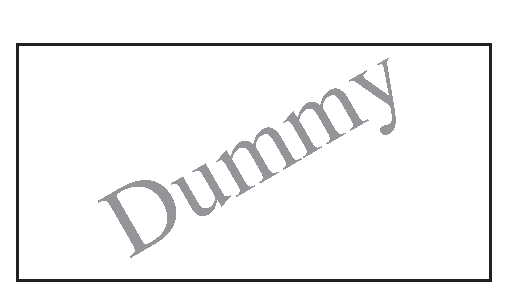
\includegraphics[width=0.5\textwidth]{img/dummy}
\caption{Utilization of four tasks on the Linux-RTXG only priority scheduling. Each tasks are given different priorities.}
\end{center}
\label{fig:rtx_prio}
\end{figure}

\begin{figure}[t]
\begin{center}
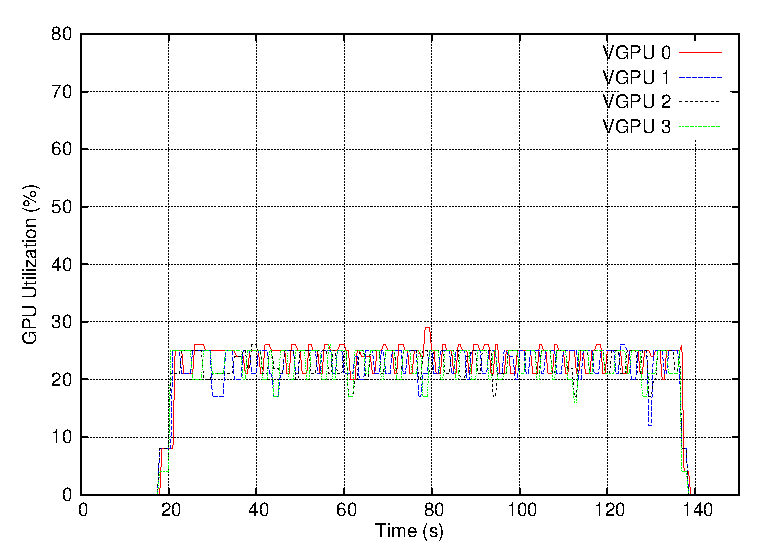
\includegraphics[width=0.5\textwidth]{img/rtx_qos.eps}
\caption{Utilization of four tasks on the Linux-RTXG resource reservation. Each tasks are given different priorities and all tasks are fairly given resources which is 25\%}
\end{center}
\label{fig:qos_rtx}
\end{figure}

\begin{figure}[t]
\begin{center}
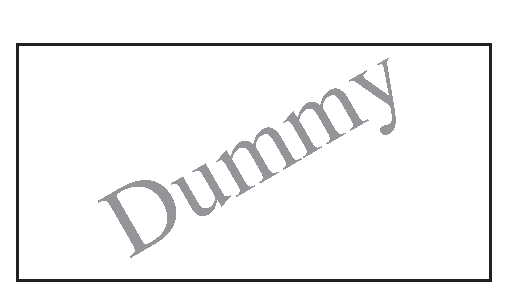
\includegraphics[width=0.5\textwidth]{img/dummy}
\caption{Utilization of four tasks on the Gdev resource resevation. All tasks are fairy given resources which is 25\%}
\end{center}
\label{fig:qos_gdev}
\end{figure}


Figure~\ref{fig:qos_gdev},\ref{fig:qos_rtx} show gpu usage on the qos management by gdev and linux-rtxg.
\TODO{結果に合わせて記述}


%%%

Figure~\ref{} shows 

\SECTION{Discussion}\label{sec:relatedwork}

Here, we discuss the comparing between proposed Linux-RTXG framework and previous study.

\begin{table*}[t]
\begin{center}
\caption{Linux-RTXG vs Prior Work}
\label{tab:comp:prior}
%\begin{tabular}{|c|c|c|c|c|c|c|c|c|c|c|} \hline
\begin{tabular}{ccccccccccc} \hline
 & CPU & CPU & GPU Prio. & Budget & Data/Comp. & Closed Src.& Kernel& OS & GPU Runtime \\ 
& FP & EDF & Sched. & Enforcement & Ovlp. & Compatible & Free & independent & independent \\ \hline
 RGEM       &   &   & x &   &   & x & x & x &   \\ 
 Gdev       &   &   & x & x & x &   &   &   &   \\ 
 PTask      &   &   & x & x & x & x &   &   & x \\ 
 GPUSync    & x & x & x & x & x & x &   &   & x \\ 
 GPUSparc   & $B"%(B &   & x &   & x & x &   & x &   \\ 
 Linux-RTXG & x & x & x & x & x & x & x & x & x \\ \hline
\end{tabular}
\end{center}
\end{table*}

RGEM and GPU-Sparc~\cite{sparc} have GPU resource management without kernel and device driver modification.
However, the synchronization mechanisms of these methods depends on proprietary-software.
TimeGraph, Gdev, Ptask, and GPUSync realize independent synchronization mechanisms that do modify the kernel and device drivers.
To the best of our knowledge, the proposed Linux-RTXG is the only real-time GPU framework that uses a synchronization mechanisms
that are independent of runtime and do not modifiy the kernel and device drivers.

Table~\ref{tab:comp:prior} shows a comparison of the proposed Linux-RTXG and previous methods.
GPU sync supports the fixed-priority and EDF CPU scheduling policies.
GPUSparc employs the $SCHED\_FIFO$ Linux scheduling policies.
Note that Linux-RTXG demonstrates all features shown in Table~\ref{tab:comp:prior}.
In particular, Linux-RTXG is both GPU runtime independendt and OS independent.

More in-depth resource management would require detailed information about the execution mechanisms in bacl--box GPU stacks.
Menychtas et al. presented enabling to GPU using OS reserach by inferring interactions in a black--box GPU stack~\cite{menychatas2013enabling}.
We have presented information about GPU microcontrollers~\cite{fujii:apsys2013} and an open-source GPGPU runtime~\cite{kato:gdev}.
In addition, GPUSync verifies proprietary runtime chanism infomation.
The Nouveau project provide an open-source GPU driver~\cite{nouveau}.

The more-depth resource management would require the detail executing mechanisms in the black-box GPU stack.
Menychtas et al. present enabling GPU using OS research by inferring interaction in the black-box GPU stack~\cite{menychtas2013enabling}.
We present information of GPU microcontrollers~\cite{fujii:apsys2013} and an open-source GPGPU runtime~\cite{kato:gdev}.
GPUSync presents details verification information on the proprietary runtime mechanisms.
Nouveau project provides an open-source GPU driver~\cite{nouveau}.
%These works are very important, and we will also views of the further development of resource management their researches.

%In order to more growth the GPU as a powerful device,
%The challenges are efficiency compler, efficiency runtime, efficiency system such as treatment PCI.

%$B2f!9$O$3$l$^$G$$$/$D$+$N(BGPU$B$N;q8;4IM}$K4X$9$k8&5f(B~\cite{kato:timegraph,kato:rtas2011,kato:rgem,kato:gdev}$B$r9T$C$F$-$?!#(B
%TimeGraph$B$O(BGPU$B$KAw?.$5$l$k%3%^%s%I$r%9%1%8%e!<%j%s%0$9$k$3$H$G(BCUDA$B$K$+$.$i$:!"(BOpenGL$B$J$I!"(B
%$BA4$F$N(BGPU$B$rMxMQ$K4X$9$k;q8;4IM}$r9T$C$F$$$k!#(B
%$B$7$+$7$J$,$i(BGPU$B$N%3%^%s%I$O=hM}$N<B9T$@$1$G$J$/!"%G!<%?E>Aw!"3d9~$_=hM}EPO?$J$I$N=hM};~$K$bAw?.$5$l$F$*$j!"(B
%$BK\Ev$K%9%1%8%e!<%j%s%0$9$k$Y$-C10L$G$N%9%1%8%e!<%j%s%0$K$O8~$$$F$$$J$$$3$H$,$o$+$C$F$$$k!#(B
%$B$=$N$?$a!"(BRGEM$B$O(BGPGPU$B$KFC2=$7!"(BGPU$B%+!<%M%k<B9TC10L$G$N%9%1%8%e!<%j%s%0$rL\;X$7!"8GDjM%@hEY$G$N%9%1%8%e!<%j%s%0$r<B8=$7$F$k!#(B
%$B2C$($F!"%G!<%?E>Aw$N%;%0%a%s%HJ,$1$K$h$C$F%N%s%W%j%(%s%W%F%#%V$JFC@-$K$b$?$i$5$l$k%G%a%j%C%H$r:G>.8B$K$7!"(B
%$B%l%9%]%s%9%?%$%`$N8~>e$rL\;X$7$F$$$k!#(B
%Gdev$B$O(BRGEM$B$NH/E87A$G$"$j!"2>A[(BGPU$B$H(BResource Reservation$B$K$h$k(BQoS$B@)8f$d!"(BOS$B6u4V$G$N(BCUDA$B<B9T$J$I$r<B8=$7$F$$$k!#(B
%$B2C$($F%G!<%?E>Aw$H%+!<%M%k<B9T$r%*!<%P%i%C%W$5$;$k$3$H$G<B9T;~4V<+BN$N=L>.$r<B8=$7$F$$$k!#(B
%
%PTask~\cite{ptask} is an OS abstraction for GPU applications that optimizes data transfers and GPU scheduler.
%
%Elliott et al. present GPUSync~\cite{elliott2013gpusync,elliott:explor14}.
%GPUSync$B$G$O%[%9%H$+$i(BGPU$B$X$N%G!<%?E>Aw3+;O$+$i!"(BGPU$B$G$N=hM}!"(BGPU$B$+$i%[%9%H$X$N%G!<%?E>Aw$^$G$r%/%j%F%#%+%k%;%/%7%g%s$H@_Dj$7!"(B
%runtime$B$X$N%"%/%;%9$O%/%j%F%#%+%k%;%/%7%g%s$r6h@Z$j$H$7$FC10l$N%"%/%;%9$H$J$k$h$&$KD4Dd$r9T$C$F$$$k!#(B
%$B$3$l$K$h$C$F%/%m!<%:%I%=!<%9$J%i%s%?%$%`$rMxMQ$7$D$D!"<+?H$N(BGPU$B;q8;4IM}$r<B8=2DG=$H$7$F$$$k!#(B
%GPUSync$B$O%"%/%;%9D4Dd$N<jK!$H$7$F(Bk-exclusion lock$B$N3HD%$rMxMQ$7$F$$$k!#(B
%$B2C$($F3F(BGPU$B$4$H$K(BResource Reservation$B$K$h$k(BQoS$BC4J]$r9T$C$F$*$j!"3F(BGPU$B4V$N(BP2P migration$B$b<B8=$7$F$*$j!"(BMultipleGPU$B$X$N<+F03d$jEv$F$b9T$C$F$$$k!#(B

%Han et al. show GPU-SPARC~\cite{sparc}.
%GPU-Sparc support to automatically split and run the GPU kernel concurrently over multi-GPU, and then they supported priority queue based scheduling.


\section{Conclusion}\label{sec:conclusion}
In this paper,
we present linux real-time extension for cpu-gpu resouce coordination is called Linux-RTXG for cpu and gpu coordinated resource management.
We focus on that are specifically not modify the kernel, worked for GPU resource management.
Linux-RTXG present the CPU task scheduling, the GPU task sheduling and the GPU resource reservation mechanisms.
The CPU task scheduling is based on RESCH.
The GPU task scheduling provides prioritized scheduling by our synchronization mechanisms.
Our synchronization mechanisms is not need to modify the kernel and device drivers, presented by intercept interrupt top-half ISRs.

\TODO{$BI>2A7k2L$K$D$$$F(B:}
\TODO{overhead:}
$B:#2s<B8=$7$?%U%l!<%`%o!<%/$O!"%8%g%V0l8D$"$?$j$N%*!<%P%X%C%I$OLs(Bx\%(sleep$B$7$F$$$k;~4V$b4^$`(B)$B$K$J$j!"(Btask$B$"$?$j$N%*!<%P%X%C%I$OLs(Bx\%$B$K<}$^$k$3$H$r<($7$?!#(B
$B2C$($F4{B8%U%l!<%`%o!<%/$G$"$k(BGdev$B$HF10l%"%k%4%j%:%`$rMQ$$$F!"3d9~$_K5D0$rMQ$$$?(BQoS Management$B$N@-G=$r8!>Z$7B?>/$N@-G=Dc2<$G<}$^$k$3$H$r3NG'$7$?!#(B
\TODO{qos management}

\TODO{$B7k2L$K$D$$$F=*$o$j(B}

The Basic frame of scheduling framework is already completion for realized real-time GPU.
In the future work, Be addressed to improvement GPU execution (preemptive, p2p migration) is essensial matter in order to more real-time framework.
%$B%j%"%k%?%$%`(BGPU$B$r<B8=$9$k$?$a$N!$%9%1%8%e!<%j%s%0%U%l!<%`%o!<%/$N4pK\%U%l!<%`$O4{$K40@.$7$?!%(B
%$B:#8e$O(BGPUSync$B$d(BGPUSparc$B$,CeL\$7$F$$$k$=$NB>(BGPU$B<B9T$K4X$9$k2~NI(B(preemptive, p2p migration)$B$J$I$K$b<h$jAH$`$3$H$G$h$j%j%"%k%?%$%`$J(BGPU$B$K6a$E$/$3$H$,$G$-$k!%(B




\appendices

% you can choose not to have a title for an appendix
% if you want by leaving the argument blank

% use section* for acknowledgement
\ifCLASSOPTIONcompsoc
  % The Computer Society usually uses the plural form
  \section*{Acknowledgments}
\else
  % regular IEEE prefers the singular form
  \section*{Acknowledgment}
\fi


The authors would like to thank...


% Can use something like this to put references on a page
% by themselves when using endfloat and the captionsoff option.
\ifCLASSOPTIONcaptionsoff
  \newpage
\fi



% trigger a \newpage just before the given reference
% number - used to balance the columns on the last page
% adjust value as needed - may need to be readjusted if
% the document is modified later
%\IEEEtriggeratref{8}
% The "triggered" command can be changed if desired:
%\IEEEtriggercmd{\enlargethispage{-5in}}

% references section

% can use a bibliography generated by BibTeX as a .bbl file
% BibTeX documentation can be easily obtained at:
% http://www.ctan.org/tex-archive/biblio/bibtex/contrib/doc/
% The IEEEtran BibTeX style support page is at:
% http://www.michaelshell.org/tex/ieeetran/bibtex/
%\bibliographystyle{IEEEtran}
% argument is your BibTeX string definitions and bibliography database(s)
%\bibliography{IEEEabrv,../bib/paper}
%
% <OR> manually copy in the resultant .bbl file
% set second argument of \begin to the number of references
% (used to reserve space for the reference number labels box)

\bibliographystyle{IEEEtranBST/IEEEtran}

\bibliography{bib/gpu_ap,bib/gpu_rm,bib/gpu,bib/os,bib/realtime}

% biography section
% 
% If you have an EPS/PDF photo (graphicx package needed) extra braces are
% needed around the contents of the optional argument to biography to prevent
% the LaTeX parser from getting confused when it sees the complicated
% \includegraphics command within an optional argument. (You could create
% your own custom macro containing the \includegraphics command to make things
% simpler here.)
%\begin{biography}[{\includegraphics[width=1in,height=1.25in,clip,keepaspectratio]{mshell}}]{Michael Shell}
% or if you just want to reserve a space for a photo:

\begin{IEEEbiography}{Yusuke Fujii}
Biography text here.
\end{IEEEbiography}
\begin{IEEEbiography}{Takuya Azumi}
Biography text here.
\end{IEEEbiography}
\begin{IEEEbiography}{Nobuhiko Nishio}
Biography text here.
\end{IEEEbiography}
\begin{IEEEbiography}{Tuyoshi Hamada}
Biography text here.
\end{IEEEbiography}
\begin{IEEEbiography}{Shinpei Kato}
Biography text here.
\end{IEEEbiography}
% You can push biographies down or up by placing
% a \vfill before or after them. The appropriate
% use of \vfill depends on what kind of text is
% on the last page and whether or not the columns
% are being equalized.

%\vfill

% Can be used to pull up biographies so that the bottom of the last one
% is flush with the other column.
%\enlargethispage{-5in}



% that's all folks
\end{document}


